\documentclass{article}
%引用设置使用Bibtex
\usepackage{gbt7714}
\bibliographystyle{gbt7714-numerical}
%页面设置
\usepackage{geometry}
%字体设置
\usepackage{fontspec}
%\setmainfont{Times New Roman}
%定理环境
\usepackage{amsmath}
\numberwithin{equation}{section}
\usepackage{amsthm}
%\newtheorem*{definition}{定义}
%\newtheorem{theorem}{定理}
%\newtheorem{lemma}{Lemma}
\newtheorem*{corollary}{推论}
\newtheorem*{proposition}{命题}
\newtheorem*{example}{例}
%数学环境字体
\usepackage{bm}
\usepackage[all]{xy}
%加载 TikZ 用于绘制交换图
\usepackage{tikz-cd}
%颜色
\usepackage{color,xcolor}

\definecolor{miku}{RGB}{57,197,187}
\definecolor{sakura}{RGB}{255,192,203}
\definecolor{rose}{RGB}{255,228,225}
\definecolor{brown}{RGB}{210,105,30}
\definecolor{lbrown}{RGB}{239,235,224}
\definecolor{bule}{RGB}{0,47,167}
\definecolor{lyellow}{RGB}{250,250,210}
\definecolor{lpurple}{RGB}{255,240,245}
\definecolor{lbule}{RGB}{135,206,250}
\definecolor{gbule}{RGB}{64,224,208}
\definecolor{green}{RGB}{138,200,207}
\definecolor{lgreen}{RGB}{225,255,255}
\definecolor{lorange}{RGB}{248,172,140}
\definecolor{salmon}{RGB}{250,128,114}
\definecolor{burgundy}{rgb}{0.5, 0.0, 0.13}
%链接设置
\usepackage[colorlinks=true,pdfstartview=FitH,linkcolor=blue,anchorcolor=violet, citecolor=magenta]{hyperref} 
%封面
\usepackage{pdfpages}
\usepackage{mathrsfs}
\usepackage{amssymb}
\usepackage{graphicx}
\usepackage{lipsum}
%彩色框
\usepackage{framed}
\usepackage{tcolorbox}
\tcbuselibrary{breakable}
\tcbuselibrary{theorems}
\tcbuselibrary{skins}
\usepackage{colortbl}
\usepackage{float}
\usepackage[export]{adjustbox}
\newtcolorbox[auto counter,number within=section]{notebox}[2][]{%
colback=miku!2!white,
colframe=miku,
coltitle=white,
fonttitle=\bfseries,
rightrule=2pt,
leftrule=2pt,
bottomrule=2pt,
colbacktitle=miku,
theorem style=standard,
breakable,
arc=2pt,
drop fuzzy shadow=black!20!white,
title=Note~\thetcbcounter: #2,#1}
\newtcolorbox[auto counter,number within=section]{markbox}[2][]{%
colback=miku!2!white,
colframe=miku,
coltitle=white,
fonttitle=\bfseries,
rightrule=0pt,
leftrule=0pt,
bottomrule=2pt,
colbacktitle=miku,
theorem style=standard,
breakable,
arc=0pt,
drop fuzzy shadow=black!20!white,
title=Remark~\thetcbcounter: #2,#1}
\newtcolorbox[no counter]{theorems}[2][]{%
width=12cm,
center,
sidebyside,
sidebyside adapt=left,
sidebyside gap=6mm,
sidebyside align=center seam,
colback=burgundy!2!white,
colframe=burgundy,
coltitle=white,
fonttitle=\bfseries,
rightrule=1pt,
leftrule=1pt,
bottomrule=2pt,
colbacktitle=burgundy,
theorem style=standard,
enhanced,
drop fuzzy shadow southeast=black!30!white,
breakable,
arc=0pt,
title=Theorem. #2,#1}
\newtcolorbox[no counter]{definitions}[2][]{%
width=12cm,
center,
colback=lyellow!2!white,
colframe=yellow!3!lyellow,
coltitle=bule,
fonttitle=\bfseries,
rightrule=0pt,
leftrule=1pt,
bottomrule=2pt,
colbacktitle=lyellow,
theorem style=standard,
breakable,
arc=5pt,
enhanced,
drop fuzzy shadow southeast=black!20!white,
title=Definition. #2,#1}
\newtcolorbox[auto counter,number within=section]{corollarys}[2][]{%
colback=lyellow!2!white,
colframe=lyellow,
coltitle=bule,
fonttitle=\bfseries,
rightrule=0pt,
leftrule=1pt,
bottomrule=2pt,
colbacktitle=lyellow,
theorem style=standard,
breakable,
arc=0pt,
enhanced,
drop fuzzy shadow southeast=black!20!white,
title=Corollary~\thetcbcounter: #2,#1}
\newtcolorbox[auto counter,number within=section]{lemmas}[2][]{%
width=12cm,
center,
colback=lyellow!2!white,
colframe=lorange!30!sakura,
coltitle=bule,
fonttitle=\bfseries,
rightrule=0pt,
leftrule=1pt,
bottomrule=2pt,
colbacktitle=lorange!30!sakura,
theorem style=standard,
breakable,
arc=5pt,
enhanced,
drop fuzzy shadow southeast=black!20!white,
title=Lemma. #2,#1}
\newtcolorbox[auto counter,number within=section]{propositions}[2][]{%
width=12cm,
center,
colback=salmon!5,
colframe=salmon!90!black,
coltitle=white,
fonttitle=\bfseries,
rightrule=1pt,
leftrule=1pt,
bottomrule=2pt,
colbacktitle=salmon!90!black,
theorem style=standard,
breakable,
arc=5pt,
enhanced,
drop fuzzy shadow southeast=black!20!white,
title=Proposition. #2,#1}
\newtcolorbox[no counter]{egbox}[2][]{%
width=12cm,
center,
colback=black!5!white,
colframe=black!20!white,
coltitle=black,
fonttitle=\bfseries,
rightrule=1pt,
leftrule=1pt,
bottomrule=2pt,
colbacktitle=black!20!white,
theorem style=standard,
breakable,
arc=0pt,
enhanced,
drop fuzzy shadow southeast=black!20!white,
title=Example. #2,#1}

%\begin{figure}[H]
%\centering
%\includegraphics[center]{pic.png}
%\end{figure}
\geometry{left=3cm,right=3cm,top=2cm,bottom=2cm}
\tcbuselibrary{most}

\usepackage[linesnumbered,ruled,vlined]{algorithm2e}
\usepackage{algorithmic}

\SetKwProg{Fn}{function}{\string:}{}
\newcommand{\forcond}{$i=0$ \KwTo $n$}
\SetKwFunction{FRecurs}{FnRecursive}
\SetKwInput{KwCost}{Cost}

\usepackage{holtpolt}

%自定义设置
\renewcommand{\proofname}{Proof.}
\renewcommand{\contentsname}{ Content }
\newcommand{\image}[2]{
    \centering
    \includegraphics[width={#1}\textwidth]{#2}
}



\newcommand\keywords[1]{\vskip2ex\par\noindent\normalfont{\textbf{关键词}: #1}}
\newcommand{\ekeywords}[1]{\vskip2ex\par\noindent\normalfont{\bfseries Key Words: }#1}
\newcommand{\miku}{\textcolor{miku}}
\newcommand{\sakura}{\textcolor{sakura}}
\newcommand{\brown}{\textcolor{brow}}
\newcommand{\red}{\textcolor{red}}
\newcommand{\blue}{\textcolor{blue}}
\newcommand{\A}{\mathcal{A}}
\newcommand{\C}{\mathbb{C}}
\newcommand{\al}{\alpha}
\newcommand{\sa}{$\sigma$-algebra}
\newcommand{\Bsa}{Borel $\sigma$-algebra}
\newcommand{\F}{\mathcal{F}}
\newcommand{\N}{\mathcal{N}}
\newcommand{\M}{\mathcal{M}}
\newcommand{\m}{ $\mathcal{M}$ }
\newcommand{\B}{\mathcal{B}}
\newcommand{\myP}{\mathcal{P}}
\renewcommand{\bf}[1]{\textbf{#1}}

\newcommand{\myRom}[1]{\uppercase\expandafter{\romannumeral#1}}
\newcommand{\pl}{$ L^p(X) $}
\newcommand{\twol}{$ L^2(X) $}

\newcommand{\Hom}{{\rm Hom}}


\usepackage{xeCJK}
\setCJKmainfont{Source Han Serif CN}
\usepackage{fontspec}
\setmainfont{Times New Roman}
% 为粗体定义 Source Han Serif CN 的粗体版本
\setCJKfamilyfont{sourcehanserifbf}{Source Han Serif CN}
\renewcommand{\bf}[1]{{\CJKfamily{sourcehanserifbf}\bfseries #1}}

\graphicspath{
    {./fig/}{./figure/}{./figures/}{./image/}{./images/}{./graphic/}{./graphics/}{./picture/}{./pictures/}
}

% 设置楷体字体
\setCJKfamilyfont{kai}{KaiTi}  % 替换为合适的楷体字体

% 定理环境中的字体设置为楷体
\newtheoremstyle{kai-theorem}  % 定义新的定理样式
  {3pt}   % 上方间距
  {3pt}   % 下方间距
  {\CJKfamily{kai}}  % 正文楷体字体
  {}      % 缩进
  {\bfseries} % 标题加粗
  {.}     % 标题后面的标点符号
  { }     % 标题和正文之间的间距
  {\thmname{#1}\thmnumber{ #2}\thmnote{ (#3)}} % 定理标题格式

% 应用新的定理样式
\theoremstyle{kai-theorem}
\newtheorem{definition}{定义}
\newtheorem{theorem}{定理}
\newtheorem{lemma}{引理}

\begin{document}
\begin{center}\huge
  \textbf{模论初步}
\end{center}
\begin{center}
  \textbf{课程:代数学(MATH5002P)}\\ \textbf{陈曦}  chenx1@mail.ustc.edu.cn 
\end{center}

\section{模的定义与基本性质}
\begin{definition}
    设$ R $是一个含幺交换环,非空集合$ M $是一个Abel群。如果$ R $关于$ M $存在一个二元运算
    \begin{equation}
        (\cdot,\cdot) : R\times M\to M,\quad (r,m)\mapsto r.m\quad (\text{ abbr. } rm) 
    \end{equation}
    使得对任意$ m,m'\in M $和$ r,r'\in R $,满足以下条件:
    \begin{enumerate}
        \item 存在恒等元:如果$ 1=1_R $是$ R $的幺元,则$ 1m=m $;
        \item 分配律成立:$ r(m+m') = rm+rm' $,$ (r+r')m = rm+r'm $;
        \item 结合律成立:$ r(r'm) = (rr')m $;
    \end{enumerate}
    则称$ (\cdot,\cdot) $是$ M $上的\bf{R乘}运算,称$ M $是一个\bf{R-模(module)},记作$ _RM $。
\end{definition}

\subsection{直积与直和}
\begin{definition}
    给定R-模$S$和$T$和某一三元组$ (M;p,q) $,其中$ p\in \Hom_R(M,S) $,$ q\in \Hom_R(M,T) $,如果关于任意的$ N\in $R-mod和$ f\in \Hom_R(N,S) $、$ g\in \Hom_R(N,T) $都存在唯一的$ \varphi\in \Hom_R(N,M) $使得图\ref{fig:moduleproduct}交换,则称$ M $是$ S $和$ T $的\bf{(外)直积(Product)},记作$ M=S\times T $。
\end{definition}
\begin{figure}[htpb]
    \centering
    \begin{tikzcd}
        &  &                                    & S \\
\forall N \arrow[rrru, "\forall f"', bend left] \arrow[rrrd, "\forall g", bend right] \arrow[rr, "\exists ! \varphi" description] &  & M = S\times T \arrow[ru, "p"'] \arrow[rd, "q"] &   \\
        &  &                                    & T
\end{tikzcd}
    \caption{(外)直积}
    \label{fig:moduleproduct}
\end{figure}
\noindent 上述定义中的要求称为“泛性质”(universal property)。一般地,如果某定义中需要考虑“在给定某些条件下存在唯一态射”这种形式的性质,则称该性质为\bf{泛性质}。

\paragraph{直积的唯一性} 如果$ M $和$ M' $都满足以上关系,从而都是$ S $和$ T $的直积,则分别使用$ M $和$ M' $的泛性质可知分别存在唯一的模同态$ \varphi:M'\to M $和$ \psi:M\to M' $使得图\ref{fig:uniqueness_of_product}交换,即
\[
    p\circ \psi = p',\quad q\circ \psi = q',\quad p'\circ \varphi = p,\quad q'\circ \varphi = q,
\]
于是
\[
    p\circ \psi\circ \varphi = p,\quad q'\circ \varphi\circ \psi = q'.
\]
上式是图\ref{fig:uniqueness_of_product}交换的必要条件。

\begin{figure}[htpb]
    \centering
    \begin{tikzcd}
        & S &                                                                   \\
M' \arrow[ru, "p'"] \arrow[rd, "q'"'] \arrow[rr, "\varphi", shift left] &   & M \arrow[lu, "p"'] \arrow[ld, "q"] \arrow[ll, "\psi", shift left] \\
        & T &                                                                  
\end{tikzcd}
    \caption{直积的唯一性}
    \label{fig:uniqueness_of_product}
\end{figure}

注意到要让上式成立等价于要求图\ref{fig:uniqueness_of_product_necessary}交换这一特殊情况,此时$ M'=M $,相应地$ p'=p,q'=q $。此时$ \phi={\rm Id}_M $显然是使得图表交换的一组模同态,又因为泛性质中要求该模同态唯一,因此
\[
    \psi\circ \varphi = {\rm Id}_M,
\]
类似地可知$ \varphi\circ \psi = {\rm Id}_{M'} $,故$ \psi $和$ \varphi $互为逆同态,进而$ M $和$ M' $同构,这就说明了直积的唯一性。

\begin{figure}[htpb]
    \centering
    \begin{tikzcd}
        & S &                                                        \\
M \arrow[ru, "p"] \arrow[rd, "q"'] &   & M \arrow[lu, "p"'] \arrow[ld, "q"] \arrow[ll, "\phi"'] \\
        & T &                                                       
\end{tikzcd}
    \caption{寻找所有可行的模同态$ \phi = \psi\circ \varphi $}
    \label{fig:uniqueness_of_product_necessary}
\end{figure}

\paragraph{直积的经典形式} 上面我们已经证明了由泛性质定义的$ S $和$ T $的所有直积在同构意义下都相同,这其中一种最常用的直积表示形式是把直积写成笛卡尔积的样式,即
\begin{equation}
    S\times T = \{(s,t)\mid s\in S,t\in T\},
\end{equation}
相应的交换图可以表示成如图\ref{fig:classical_product}的形式,其中$ \pi_1 $和$ \pi_2 $分别是$ S\times T $到$ S $和$ T $的\bf{典范投射},即
\[
    \pi_1(s,t) = s,\quad \pi_2(s,t) = t.
\]
在这种情况下泛性质要求
\[
    f = \pi_1\circ \varphi,\quad g = \pi_2\circ \varphi,
\]
将两边都作用在$ x\in N $上可得
\[
    f(x) = \pi_1(\varphi(x)),\quad g(x) = \pi_2(\varphi(x)),
\]
令$ \varphi(x) = (s_x,t_x) $,于是
\[
    f(x) = s_x,\quad g(x) = t_x,
\]
因此
\begin{equation}
    \varphi(x) = (f(x),g(x)).
\end{equation}
于是我们再一次看到$ f,g $唯一决定了$ \varphi $,由此也可见$ \varphi $的至多唯一性。
通常我们习惯上将$ S\times T $中的元素写成列向量的形式,以便将$ \varphi $写为简洁的算子形式,即
\begin{equation}
    \varphi = \begin{pmatrix}
        f \\ g
    \end{pmatrix}
    \text{ i.e. }
    \varphi(x) = \begin{pmatrix}
        f(x) \\ g(x)
    \end{pmatrix}.
\end{equation}

\begin{figure}[htpb]
    \centering
    \begin{tikzcd}
        & S &                                                    \\
N \arrow[ru, "f"] \arrow[rd, "g"'] \arrow[rr, "\varphi=\begin{pmatrix}
    f \\ g
\end{pmatrix}" description] &   & S\times T \arrow[lu, "\pi_1"'] \arrow[ld, "\pi_2"] \\
        & T &                                                   
\end{tikzcd}
    \caption{直积的经典表示}
    \label{fig:classical_product}
\end{figure}

与直积相应的概念称为直和,模的直和应当满足的泛性质对应的交换图\ref{fig:modulecoproduct}中的各箭头与直积的交换图\ref{fig:moduleproduct}中的各箭头方向相反。在范畴上直积和直和是互相对偶的两个概念。
\begin{definition}
    给定R-模$S$和$T$和某一三元组$ (M;p,q) $,其中$ p\in \Hom_R(M,S) $,$ q\in \Hom_R(M,T) $,如果关于任意的$ N\in $R-mod和$ f\in \Hom_R(S,N) $、$ g\in \Hom_R(T,N) $都存在唯一的$ \psi\in \Hom_R(M,N) $使得图\ref{fig:modulecoproduct}交换,则称$ M $是$ S $和$ T $的\bf{(内)直和(Coproduct)},记作$ M=S\oplus T $。
\end{definition}

\begin{figure}[htpb]
    \centering
    \begin{tikzcd}
        &  &                                            & S \arrow[ld, "i"] \arrow[llld, "\forall f", bend right] \\
\forall N &  & M = S\oplus T \arrow[ll, "\exists ! \psi" description] &                                                         \\
        &  &                                            & T \arrow[lu, "j"'] \arrow[lllu, "\forall g"', bend left]
\end{tikzcd}
    \caption{(内)直和}
    \label{fig:modulecoproduct}
\end{figure}

与直积类似,我们可以说明由上述泛性质定义的直和在同构意义下是唯一的。另外,最经典的刻画直和的方式是使用唯一分解,即如果$ S,T $都是$ M $的子模,并且满足
\begin{equation}
    M = S+T,\quad S\cap T = \{0\},
\end{equation}
则称$ M $是$ S $和$ T $的直和,记作$ M=S\oplus T $。这种刻画方式下,直和的泛性质可以表示成如图\ref{fig:classical_coproduct}的形式,其中$ i_1 $和$ i_2 $分别是$ S $和$ T $到$ M $的\bf{典范嵌入},即
\[
    i_1(s) = (s,0),\quad i_2(t) = (0,t).
\]
使用泛性质可知
\[
    f = \psi\circ i_1,\quad g = \psi\circ i_2,
\]
于是
\[
    f(s) = \psi(s,0),\quad g(t) = \psi(0,t),
\]
进而
\begin{equation}
    \psi(s,t) = \psi(s,0) + \psi(0,t) = f(s) + g(t).
\end{equation}
与直积对应,我们将$ S\oplus T $内的元素写为列向量形式,于是$ \psi $可以写为算子形式,即
\begin{equation}
    \psi = \begin{pmatrix}
        f & g
    \end{pmatrix}
    \text{ i.e. }
    \psi(s,t) = 
    \begin{pmatrix} 
        f & g 
    \end{pmatrix} 
    \begin{pmatrix} 
        s\\t 
    \end{pmatrix} = f(s) + g(t).
\end{equation}

\begin{figure}[htpb]
    \centering
    \begin{tikzcd}
        & S \arrow[rd, "i_1"] \arrow[ld, "f"'] &                                  \\
      N &                                      & S\oplus T \arrow[ll, "{\psi=(f,g)}" description] \\
        & T \arrow[lu, "g"] \arrow[ru, "i_2"'] &                                 
      \end{tikzcd}
    \caption{直和的经典表示}
    \label{fig:classical_coproduct}
\end{figure}

\paragraph{直积与直和的等价性}
如果$ S,T $具有直和$ S\oplus T $,则$ S\oplus T $与它们的直积$ S\times T $同构,这只需说明直积$ S\times T $满足直和的泛性质,证明依赖于交换图\ref{fig:product_is_coproduct},其中$ i_1 $和$ i_2 $分别是$ S $和$ T $到$ S\times T $的典范嵌入,即
\[
    i_1(s) = (s,0),\quad i_2(t) = (0,t),
\]
于是对任意$ f\in \Hom_R(S,N) $和$ g\in \Hom_R(T,N) $,我们有
\[
    f = \psi\circ i_1,\quad g = \psi\circ i_2,
\]
于是
\[
    \psi(s,t) = f(s) +g(t)
\]
满足直和的泛性质,故$ S\times T $是$ S $和$ T $的直和,进而根据直和的唯一性,$ S\times T $与$ S\oplus T $同构。

\begin{figure}[htpb]
    \centering
    \begin{tikzcd}
        &  &                              & S \arrow[ld, "i_1", hook] \arrow[llld, "\forall f", bend right] \\
\forall N &  & S\times T \arrow[ll, "\psi"] &                                                                 \\
        &  &                              & T \arrow[lu, "i_2"', hook] \arrow[lllu, "\forall g"', bend left]
\end{tikzcd}
    \caption{模直积与模直和同构}
    \label{fig:product_is_coproduct}
\end{figure}

\paragraph{无限个模的直积和直和}
以上我们说明了两个模的直积和直和是等价的,对于一般的$ n $个模的直积和直和可以递推地定义并证明其等价性,但是当考虑任意个模的直积和直和时,情况变得有些不同,我们定义$ \{S_\alpha\}_{\alpha\in I} $的直积为$ (M;M\stackrel{\pi_\alpha}{\longrightarrow}S_\alpha,\alpha\in I) $,它对于任意模同态族$ \{f_\alpha:N\to S_\alpha\}_{\alpha\in I}$都存在唯一的同态$ \varphi:N\to M $使得$ f_\alpha = \pi_\alpha\circ \varphi $对任意$ \alpha\in I $成立。类似地,我们定义$ \{S_\alpha\}_{\alpha\in I} $的直和为$ (M;S_\alpha\stackrel{i_\alpha}{\longrightarrow}M,\alpha\in I) $,它对于任意模同态族$ \{f_\alpha:S_\alpha\to N\}_{\alpha\in I} $都存在唯一的同态$ \psi:M\to N $使得$ f_\alpha = \psi\circ i_\alpha $对任意$ \alpha\in I $成立。

与有限情形类似,$ \{S_\alpha\}_{\alpha\in I} $的直积和直和至多唯一。直积最常用的形式仍然是笛卡尔积的形式,即
\begin{equation}
    \prod_{\alpha\in I}S_\alpha = \{(s_\alpha)_{\alpha\in I}\mid s_\alpha\in S_\alpha\},\quad \pi_\alpha: (s_\alpha)_{\alpha\in I}\mapsto s_\alpha.
\end{equation}
直和的定义与之前相比发生了改变,必须要求$ (s_\alpha)_{\alpha\in I} $中只有有限个$ s_\alpha $非零,即
\begin{equation}
    \bigoplus_{\alpha\in I}S_\alpha = \{(s_\alpha)_{\alpha\in I}\in \prod_{\alpha\in I}S_\alpha\mid s_\alpha\in S_\alpha,s_\alpha=0 \text{ holds for almost every } \alpha\in I\},\quad i_\alpha: s_\alpha\mapsto (s_\beta)_{\beta\in I},
\end{equation}
由此可见,无限情形下直积与直和的等价性不再成立,一般直积要比直和更大。

\paragraph{直和项:可以看作直和的子模} 现在给定某一个模$ M $,考察它的哪些子模可以与另一子模通过直和得到$ M $本身。
\begin{definition}
    给定R-模$ M $,$ S $是$ M $的子模。如果存在$ M $的另一个子模$ T $使得
    \begin{equation}
        M = S\oplus T,
    \end{equation}
    则称$ S $是$ M $的一个\bf{直和项}。
\end{definition}
不难证明,$ S $是$ M $的直和项当且仅当存在R-模同态$ p:M\to S $使得
\begin{equation}
    p|_S = {\rm Id}_S,
\end{equation}
这一模同态称为$ M $到$ S $的\bf{收缩}。正向只需使用直和的泛性质,反向可以验证$ T=\ker p $满足$ M = S\oplus T $。

\subsection{正合列}
\begin{lemma}\bf{Snake Lemma}
    行交换图表\ref{fig:row_communitive}诱导如下正合列:
    \begin{equation}
        \ker d' \stackrel{f_*}{\longrightarrow} \ker d \stackrel{g_*}{\longrightarrow} \ker d'' \stackrel{\delta}{\longrightarrow} {\rm coker}\ d' \stackrel{f^*}{\longrightarrow} {\rm coker}\ d \stackrel{g^*}{\longrightarrow} {\rm coker}\ d''.
    \end{equation}
    完整交换图如图\ref{fig:snake}所示。
\end{lemma}
\begin{figure}[htpb]
    \centering
    \begin{tikzcd}
        & X' \arrow[r, "f"] \arrow[d, "d''"'] & X \arrow[r, "g"] \arrow[d, "d"] & X'' \arrow[r] \arrow[d, "d'"] & 0 \\
0 \arrow[r] & Y' \arrow[r, "p"]                   & Y \arrow[r, "q"]                & Y''                           &  
\end{tikzcd}
    \caption{行正合交换图}
    \label{fig:row_communitive}
\end{figure}

\begin{figure}[htpb]
    \centering
    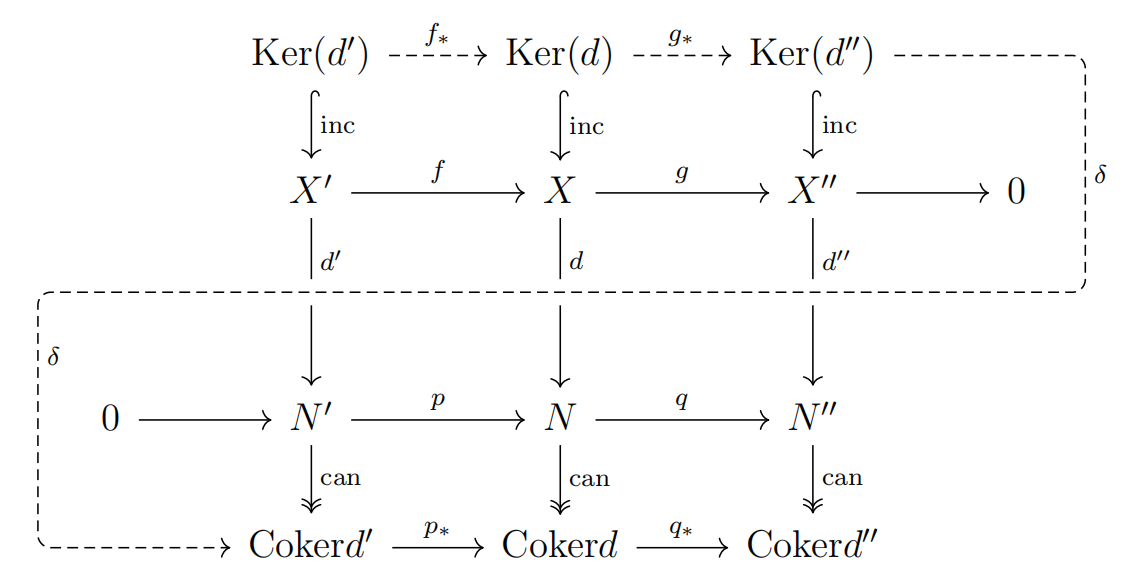
\includegraphics[width=0.6\textwidth]{SnakeLemma.png}
    \caption{蛇形引理}
    \label{fig:snake}
\end{figure}

\section{范畴论基础}
\begin{definition}
    \bf{范畴(Category)}是指一个数学系统$ \mathcal{C} $,它具有如下资料:
    \begin{enumerate}
        \item Obj($ \mathcal{C} $):其中的元素称为$ \mathcal{C} $的\bf{对象(Object)};
        \item Mor($ \mathcal{C} $):其中的元素称为$ \mathcal{C} $的\bf{态射(Morphism)},配上一对映射
        \begin{equation}
            \text{Mor}(\mathcal{C}) \xrightarrow[\quad s\quad]{t}  \text{Obj}(\mathcal{C}),
        \end{equation}
        其中$ s $和$ t $分别给出态射的\bf{来源}和\bf{目标}。对于$ X,Y\in \text{Obj}(\mathcal{C}) $,一般记$ \Hom_{\mathcal{C}}(X,Y) = s^{-1}(X)\cap t^{-1}(Y) $为从$ X $到$ Y $的态射集合,简记为$ \Hom(X,Y) $;
        \item 任意对象$ X\in \text{Obj}(\mathcal{C}) $都有一个\bf{恒等态射}$ 1_X\in \Hom(X,X) $;
        \item 任意三个对象$ X,Y,Z\in \text{Obj}(\mathcal{C}) $,它们之间的\bf{合成映射}为
        \begin{equation}
            \circ:\Hom(X,Y)\times \Hom(Y,Z)\to \Hom(X,Z),\quad (f,g)\mapsto g\circ f,
        \end{equation}
        当不会发生混淆时,通常将$ g\circ f $简记为$ gf $。这一合成满足:
        \begin{enumerate}
            \item 两两不交性:$ \Hom(X,Y) $与$ \Hom(X',Y') $交集非空当且仅当$ X=X' $且$ Y=Y' $;
            \item 结合律成立:任意态射$ h,g,f\in \text{Mor}(\mathcal{C}) $,如果$ f(gh) $和$ (fg)h $都有定义,则
            \[
                f(gh) = (fg)h,  
            \]
            \item 存在单位元:对于任意$ f\in \Hom(X,Y) $,有
            \[
                1_Yf = f1_X = f.
            \]
        \end{enumerate}
    \end{enumerate}
\end{definition}

\subsection{泛性质}
之前我们已经看到在模范畴中使用泛性质可以唯一地刻画模直积和模直和,事实上,许多代数结构可以使用泛性质来唯一地刻画,为了说明这件事需要范畴中两个特殊的对象,即终对象和始对象。
\begin{definition}
    给定范畴$ \mathcal{C} $,如果存在一个对象$ X\in \text{Obj}(\mathcal{C}) $,对于任意$ Y\in \text{Obj}(\mathcal{C}) $,$ \Hom(X,Y) $内都只有一个元素,则称$ X $是$ \mathcal{C} $的\bf{始对象};如果$ \Hom(Y,X) $内都只有一个元素,则称$ X $是$ \mathcal{C} $的\bf{终对象}。如果某对象既是始对象又是终对象,则称它是\bf{零对象}。
\end{definition}
注意到如果$ X $是$ \mathcal{C} $的始对象,则$ \Hom(X,X)=\{1_X\} $,如果$ X' $也是$ \mathcal{C} $的始对象,设$ \Hom(X,X') = \{\varphi\} $,$ \Hom(X',X)=\{\psi\} $,则$ \varphi\circ \psi = 1_X $,$ \psi\circ \varphi = 1_{X'} $,于是$ \varphi $和$ \psi $是$ X $和$ X' $之间的同构,这说明始对象在同构意义下是至多唯一的。同理可知终对象至多唯一。不过一般而言,始对象和终对象不一定存在。
\begin{definition}
    如果$ \mathcal{C} $有零对象$ 0 $,则对任意的$ X,Y\in \text{Obj}(\mathcal{C}) $可以定义其\bf{零态射}为$ \Hom(X,0) $内态射与$ \Hom(0,Y) $内态射的合成,即
    \begin{equation}
        0_{X,Y} = 0_{0,Y}\circ 0_{X,0}:X\to 0\to Y,
    \end{equation}
    其中$ 0_{X,0} $和$ 0_{0,Y} $分别是$ \Hom(X,0) $和$ \Hom(0,Y) $内唯一的元素。
\end{definition}

\section{自由模、投射模与内射模}

\end{document}